\documentclass{beamer}
\usepackage[utf8]{inputenc}

\usepackage{amsmath}
\usepackage{graphicx}
\usepackage{url}
\usepackage{fancyvrb}
\usepackage{xcolor}

\usetheme{Antibes}
\usecolortheme{whale}
\usepackage{lmodern}

\usepackage{listings}
\usepackage{color}

\definecolor{codegreen}{rgb}{0,0.6,0}
\definecolor{codegray}{rgb}{0.5,0.5,0.5}
\definecolor{codepurple}{rgb}{0.58,0,0.82}
\definecolor{backcolour}{rgb}{0.95,0.95,0.92}

\mode<presentation>

\definecolor{orange}{HTML}{BC2E07}

\usepackage{hyperref}
\hypersetup{
    colorlinks,
    linkcolor=orange,
    urlcolor=blue
}

\lstdefinestyle{mystyle}{
    language=C++,
    basicstyle=\ttfamily\footnotesize,
    backgroundcolor=\color{backcolour},
    commentstyle=\color{codegreen},
    keywordstyle=\color{magenta},
    numberstyle=\tiny\color{codegray},
    stringstyle=\color{codepurple},
    breakatwhitespace=false,
    breaklines=true,
    captionpos=b,
    keepspaces=true,
    numbers=left,
    numbersep=5pt,
    showspaces=false,
    showstringspaces=false,
    showtabs=false,
    tabsize=2
}

\title{Lab \# 6: More Loops}
\subtitle{EC-102 -- Computer Systems and Programming}

\author{Usama Wajhi}
\institute{School of Mechanical and Manufacturing Engineering (SMME), \\ National University of Sciences and Technology (NUST)}
\date{\today}

\begin{document}
\begin{frame}
    \titlepage
\end{frame}

\begin{frame}
    \frametitle{Outline}
        \tableofcontents
\end{frame}

\begin{frame}
    \frametitle{The \texttt{while} Loop}
    \section{The \texttt{while} Loop} % (fold)
    \label{sec:the_while_loop}
    \subsection{Importance} % (fold)
    \label{sub:importance_while}
    \begin{columns}
        \column{0.5\textwidth}
        \begin{itemize}
            \item The \texttt{for} loop does something a fixed number of times
            \item What happens if we don't know how many times are we going to do something before we start the loop?
        \end{itemize}
        \column{0.5\textwidth}
        \begin{figure}
            \centering
            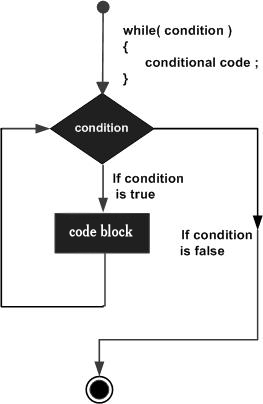
\includegraphics[scale=0.45]{while}
        \end{figure}
    \end{columns}
\end{frame}

\begin{frame}[fragile]
    \frametitle{The \texttt{while} Loop -- Syntax}
    \subsection{Syntax} % (fold)
    \label{sub:while_syntax}
    \begin{columns}
        \column{0.35\textwidth}
        \lstset{style=mystyle}
\begin{lstlisting}
while(test)
    {
       statement;
       statement;
       statement;
       statement;
    }
\end{lstlisting}
        \column{0.65\textwidth}
            \begin{itemize}
            \item Keyword \texttt{while} followed by a pair of parentheses that contain a test expression
            \item Although there is no initialization expression, the loop variable must be initialized before the loop begins
            \item The body of the loop, delimited by the left and right braces, is the code to be executed each time through the loop
            \item Similarly, the loop body must also contain some statement that keeps updating the value of the loop variable
            \end{itemize}
    \end{columns}
\end{frame}

\begin{frame} [fragile]
    \frametitle{The \texttt{while} Loop -- Solved Example 1}
    \subsection{Solved Examples} % (fold)
    \label{sub:while_solved_examples}
    \subsubsection{Solved Example 1} % (fold)
    \label{subsub:while_solved_example_1}
    \lstset{style=mystyle}
    \begin{lstlisting}
// demonstrates WHILE loop
#include <iostream>
using namespace std;
int main(){
    int num, endOfLoop = -1;
    cout << "Enter a number: ";
    cin >> num;
    
    while(num != endOfLoop){
        if(num % 2 == 0)
            cout << "The number is even.\n";
        else
            cout << "The number is odd.\n";
        cout << "Enter a number: ";
        cin >> num;
    }
    return 0;
}
\end{lstlisting}
\end{frame}

\begin{frame} [fragile]
    \frametitle{The \texttt{while} Loop -- Solved Example 2}
    \begin{columns}
        \column{0.67\textwidth}
        \lstset{style=mystyle}
\begin{lstlisting}
// sum using while loop
#include <iostream>
using namespace std;

int main(){
    int num, sum = 0;
    cout << "Enter a number: ";
    cin >> num;

    while(num != -1){
        sum = sum + num;

        cout << "Enter a number: ";
        cin >> num;
    }
    cout << "Sum = " << sum << endl;
    return 0;
}
\end{lstlisting}
        \column{0.3\textwidth}
            \begin{figure}
                \centering
                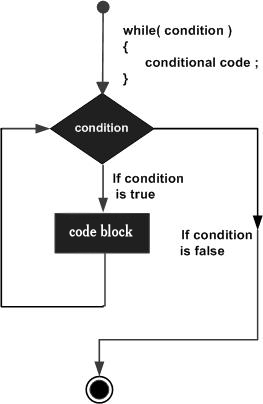
\includegraphics[scale=0.4]{while}
            \end{figure}
    \end{columns}
\end{frame}

\begin{frame} [fragile]
    \frametitle{Exercise}
    \subsection{Exercise} % (fold)
    \label{subsec:while_exercise}
    Write a calculator using \texttt{while} loop which keeps on getting a number and an operator as an input until `q' is entered as an operator. As soon as `q' is entered, the total result of the calculation is displayed and the execution of the program is stopped. \\ [0.2 in]
    Here goes a sample interaction with the program: \\
    \lstset{style=mystyle}
\begin{lstlisting}
Number: 5
Operator: +
Number: 5
Operator: *
Number: 3
Operator: -
Number: 2
Operator: /
Number: 2
Operator: q

Answer = 14
\end{lstlisting}
\end{frame}

\end{document}